\documentclass{article}
\usepackage[utf8]{inputenc}
\usepackage[sort&compress,numbers]{natbib} 
\usepackage{url}
\usepackage{hyperref} 
\usepackage{graphicx} % poner figuras
\usepackage[spanish,es-tabla]{babel} % nombre tablas
\usepackage[usenames,dvipsnames]{color}
\definecolor{deepblue}{rgb}{0,0,0.5}
\definecolor{deepred}{rgb}{0.6,0,0}
\definecolor{deepgreen}{rgb}{0,0.5,0}
\usepackage{listings}


\newcommand\pythonstyle{\lstset{
language=Python,
basicstyle=\ttm,
morekeywords={self},              % Add keywords here
keywordstyle=\ttb\color{deepblue},
emph={MyClass,__init__},          % Custom highlighting
emphstyle=\ttb\color{deepred},    % Custom highlighting style
stringstyle=\color{deepgreen},
frame=tb,                         % Any extra options here
showstringspaces=false
}}

\lstnewenvironment{python}[1][]
{
\pythonstyle
\lstset{#1}
}
{}


\lstset{ 
  language=R,                     % the language of the code
  basicstyle=\tiny\ttfamily, % the size of the fonts that are used for the code
  numbers=left,                   % where to put the line-numbers
  numberstyle=\tiny\color{Blue},  % the style that is used for the line-numbers
  stepnumber=1,                   % the step between two line-numbers. If it is 1, each line
                                  % will be numbered
  numbersep=5pt,                  % how far the line-numbers are from the code
  backgroundcolor=\color{white},  % choose the background color. You must add \usepackage{color}
  showspaces=false,               % show spaces adding particular underscores
  showstringspaces=false,         % underline spaces within strings
  showtabs=false,                 % show tabs within strings adding particular underscores
  frame=single,                   % adds a frame around the code
  rulecolor=\color{black},        % if not set, the frame-color may be changed on line-breaks within not-black text (e.g. commens (green here))
  tabsize=2,                      % sets default tabsize to 2 spaces
  captionpos=b,                   % sets the caption-position to bottom
  breaklines=true,                % sets automatic line breaking
  breakatwhitespace=false,        % sets if automatic breaks should only happen at whitespace
  keywordstyle=\color{RoyalBlue},      % keyword style
  commentstyle=\color{YellowGreen},   % comment style
  stringstyle=\color{ForestGreen}      % string literal style
} 

\title{Tarea 3: Teoría de colas}
\author{Eduardo Navarro}
\date{Septiembre 2021}

\begin{document}

\maketitle

\section{Introducción}
Con lo visto en clase se procedió a analizar los resultados obtenidos a partir de un código dado a partir de los tiempos, paro lo cual se realizaron pruebas estadísticas.

\section{Desarrollo}

Se siguieron las indicaciones de la tarea \cite{colas} a realizar primero utilizando el código en Python para producir los datos con los que se va a trabajar, del código mostrado en clase\cite{youtubesimu} se le modifico el número de núcleos que se iban a ocupar de 4 a 3 por limitaciones técnicas del equipo donde se está realizando esta tarea. se procedió a añadir pandas \cite{pandas} para un \texttt{Data.Frame} instalando la librería mediante pip y posterior mente a generar el archivo xlsx. debido a complicaciones a la hora de la recolección se decidió transferir solamente la información a una hoja de Excel para su posterior tratamiento e importación a R donde se realizará el análisis de esta información generada en Python.

\vspace{5mm}
\begin{python}
import pandas as pd ...
  paths = [] 
  for trabajadores in range (1, 4): ...
   paths.append({'replica':replica,
   'trabajadores':trabajadores,'dificultad':[label],
   'tiempo':tiempo})
   df = pd.DataFrame(paths)
 print(df)
 df.to_excel('test.xlsx', sheet_name='sheet1',
 index=False)
\end{python}
\vspace{5mm}

Como se ve en la tabla \ref{tabla1} se tiene la información ordenada donde se muestra la réplica, el número de núcleos (trabajadores), la dificultad y el tiempo que tardo en resolver

\begin{table}[h!]
\begin{center}
\caption{Ejemplo de valores obtenidos de Python}
\label{tabla1}
\begin{tabular}{|l|l|l|l|}
\hline
\multicolumn{1}{|c|}{\textbf{replica}} & \multicolumn{1}{c|}{\textbf{trabajadores}} & \multicolumn{1}{c|}{\textbf{dificultad}} & \multicolumn{1}{c|}{\textbf{tiempo}} \\ \hline
1 & 1 & fp & 4.35805321 \\ \hline
2 & 1 & fp & 4.72307205 \\ \hline
3 & 1 & fp & 5.02586365 \\ \hline
4 & 1 & fp & 4.13823128 \\ \hline
5 & 1 & fp & 5.03611565 \\ \hline
6 & 1 & fp & 4.10628319 \\ \hline
7 & 1 & fp & 4.09960747 \\ \hline
8 & 1 & fp & 4.01854515 \\ \hline
9 & 1 & fp & 4.13656235 \\ \hline
\end{tabular}
\end{center}
\end{table}

Ya en R se utilizaron las gráficas de caja bigote \ref{grafica1} para una mejor apreciación de la información donde se muestra el número de núcleos a diferentes dificultades y los intervalos de tiempo que tardaron en resolver.

\begin{figure} [h!]% figura
\renewcommand{\figurename}{Grafica}
    \centering
    \caption{Relación entre el tiempo y el número de núcleos (trabajadores)}
    \label{grafica1}
    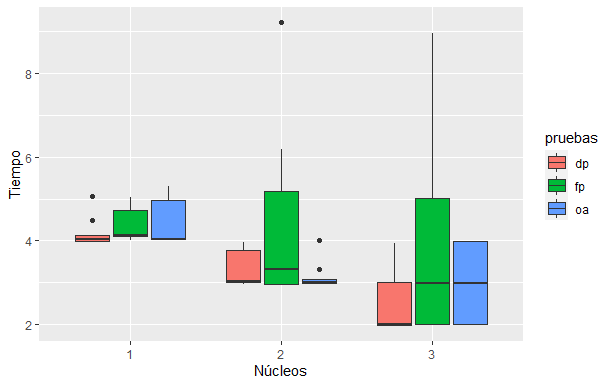
\includegraphics[width=120mm]{grafica1.png} % archivo
\end{figure}

Se procedio realizar las pruebas estadisticas utilizando la prueba de normalidad de shapiro-Wilk \cite{shapiro} con \texttt{shapiro.test} que está recomendado para muestras pequeñas, obteniendose valores en la tabla \ref{tablaSha} de p < al 0.05 lo que indica que nuestra muestra no cuenta con valores mayores al 5\% y por lo tanto no sigue una distribución normal y se rechaza la hipótesis nula, por lo que se opto por una prueba no paramétrica como la de Kruskall-Wallis\cite{Kruskall} para varias variables donde también se obtuvieron valores menores al 5\% en algunos casos.

\begin{table}[h!]
\centering
\caption{Valores obtenidos de pruebas Shapiro–Wilk}
\label{tablaSha}
\begin{tabular}{|l|r|r|}
\hline
\textbf{Shapiro} & \multicolumn{1}{l|}{W} & \multicolumn{1}{l|}{p-value} \\ \hline
Todos los datos & 0.82794 & 2.73E-08 \\ \hline
Todas las pruebas 1 núcleo & 0.75755 & 2.74E-05 \\ \hline
1 núcleo prueba fp & 0.79808 & 0.01941 \\ \hline
1 núcleo prueba dp & 0.66098 & 0.0004963 \\ \hline
Todas las pruebas 2 núcleos & 0.55607 & 6.57E-08 \\ \hline
2 núcleos prueba fp & 0.7685 & 0.008876 \\ \hline
2 núcleos prueba dp & 0.70586 & 0.001662 \\ \hline
Todas las pruebas 3 núcleos & 0.69047 & 2.87E-06 \\ \hline
3 núcleos prueba fp & 0.78479 & 0.01367 \\ \hline
3 núcleos prueba dp & 0.78479 & 0.01367 \\ \hline
Prueba fp todos los núcleos & 0.8592 & 0.001761 \\ \hline
Prueba dp todos los núcleos & 0.90071 & 0.01388 \\ \hline
Prueba oa todos los núcleos & 0.91195 & 0.02537 \\ \hline
\end{tabular}
\end{table}
En la tabla \ref{tablakrus} se pueden apreciar los diversos valores obtenidos de la prueba Kruskall-Wallis de la cual podemos inferir que tanto los valores de todos los núcleos contenidos en todas las pruebas como los de las pruebas dp y oa presentan una p < 0.05 lo que nos quiere decir que no todas las medianas de los grupos son iguales lo cual concuerda con nuestro grafico ya que los grupos de dp y oa fueron los que presentaron mayor cambio en tiempos en cuanto al número de núcleos utilizados dentro de este grupo de datos. en cuanto al grupo fp se considera que no hubo mucho cambio a la hora de medir entre núcleos en comparación con los otros dos grupos de pruebas.

\begin{table}[h!]
\centering
\caption{Valores obtenidos de pruebas Kruskal-Wallis}
\label{tablakrus}
\begin{tabular}{|l|r|r|}
\hline
Kruskall & \multicolumn{1}{l|}{H(2)} & \multicolumn{1}{l|}{p-value} \\ \hline
Todos los núcleos en todas las pruebas & 31.803 & 1.24E-07 \\ \hline
Todas las pruebas en todos los núcleos & 4.4068 & 0.1104 \\ \hline
Todas las pruebas 1 núcleo & 2.5572 & 0.2784 \\ \hline
Todas las pruebas 2 núcleos & 0.32373 & 0.8506 \\ \hline
Todas las pruebas 3 núcleos & 2.1945 & 0.3338 \\ \hline
Prueba fp todos los núcleos & 1.8765 & 0.3913 \\ \hline
Prueba dp todos los núcleos & 19.305 & 6.43E-05 \\ \hline
Prueba oa todos los núcleos & 17.648 & 0.0001471 \\ \hline
\end{tabular}
\end{table}

Código en R:

\vspace{5mm}
\begin{lstlisting}[language=R]
library(ggplot2)
library(tidyr)
library(nortest)
library(car)

datos = data.frame(
  "nucleos" = rep(c(1,2,3), times=c(27,27,27)),
  "pruebas" = rep(c("fp","dp","oa","fp","dp","oa","fp","dp","oa"), times=c(9,9,9,9,9,9,9,9,9)),
  "tiempo" = c(4.35805320739746,	4.72307205200195,	5.02586364746093,
               4.13823127746582,	5.0361156463623,	4.10628318786621,
               4.09960746765136,	4.01854515075683,	4.1365623474121, 
               4.11248207092285,	4.12225723266601,	4.47821617126464,	
               3.98898124694824,	4.02450561523437,	3.98874282836914,	
               5.0663948059082,	3.98850440979003,	4.02402877807617,	
               5.29384613037109,	4.96077537536621,	4.03094291687011, 
               4.96768951416015,	4.0135383605957,	4.01735305786132,	
               4.98390197753906,	4.02259826660156,	4.02450561523437,	
               2.95448303222656, 9.22441482543945,	6.18577003479003,	
               5.18536567687988,	4.23479080200195,	3.31377983093261,	
               2.94828414916992,	2.9611587524414, 2.95948982238769,	
               3.07941436767578,	3.76391410827636,	2.9611587524414,	
               3.0219554901123,	2.96616554260253,	3.96370887756347, 
               2.99429893493652,	2.99501419067382,	3.96418571472167,	
               4.00257110595703,	2.9914379119873,	3.00812721252441,	
               3.32427024841308, 2.95591354370117,	2.99310684204101,	
               3.07750701904296,	3.00145149230957,	2.9921531677246,	
               2.9919147491455,	8.01825523376464, 8.96430015563964,	
               5.00655174255371,	3.05914878845214,	2.99239158630371,	
               1.96743011474609,	1.99532508850097,	2.00200080871582, 
               3.93295288085937,	1.95908546447753,	1.96599960327148,	
               3.00574302673339,	2.99263000488281,	1.99532508850097,	
               1.97935104370117, 1.99556350708007,	3.00526618957519,	
               3.99065017700195,	2.9919147491455,	3.98612022399902,	
               1.99389457702636,	2.9916763305664, 1.99437141418457,	
               2.99310684204101,	3.98993492126464,	1.99413299560546)
)

datos\$nucleos = as.factor(datos\$nucleos)
datos\$pruebas = as.factor(datos\$pruebas)

ggplot(datos, aes(x= nucleos, y= tiempo, fill= pruebas)) + # fill=name allow to automatically dedicate a color for each group
  geom_boxplot()+ labs(x="Núcleos", y= "Tiempo")

shapiro.test(datos\$tiempo)

kruskal.test(tiempo~nucleos, data=datos)
kruskal.test(tiempo~pruebas, data=datos)


datos1a = data.frame( \#Todas las pruebas 1 núcleo)
  "nucleos" = rep(c(1), times=c(27)),
  "pruebas" = rep(c("fp","dp","oa"), times=c(9,9,9)),
  "tiempo" = c(4.35805320739746,	4.72307205200195,	5.02586364746093,
               4.13823127746582,	5.0361156463623,	4.10628318786621,
               4.09960746765136,	4.01854515075683,	4.1365623474121,
               4.11248207092285,	4.12225723266601,	4.47821617126464,
               3.98898124694824,	4.02450561523437,	3.98874282836914,
               5.0663948059082,	3.98850440979003,	4.02402877807617,	
               5.29384613037109,	4.96077537536621,	4.03094291687011,
               4.96768951416015,	4.0135383605957,	4.01735305786132,	
               4.98390197753906,	4.02259826660156,	4.02450561523437
  ))
shapiro.test(datos1a\$tiempo)

kruskal.test(tiempo~pruebas, data=datos1a)

datosfpa = data.frame( \# prueba fp todos los núcleos
  "nucleos" = rep(c(1,2,3), times=c(9,9,9)),
  "pruebas" = rep(c("fp"), times=c(27)),
  "tiempo" = c(4.35805320739746,	4.72307205200195,	5.02586364746093,
               4.13823127746582,	5.0361156463623,	4.10628318786621,	
               4.09960746765136,	4.01854515075683,	4.1365623474121, 
               2.95448303222656,	9.22441482543945,	6.18577003479003,	
               5.18536567687988,	4.23479080200195,	3.31377983093261,	
               2.94828414916992,	2.9611587524414,	2.95948982238769, 
               2.9919147491455,	8.01825523376464,	8.96430015563964,	
               5.00655174255371,	3.05914878845214,	2.99239158630371,	
               1.96743011474609,	1.99532508850097,	2.00200080871582

 ))

shapiro.test(datosfpa\$tiempo)

kruskal.test(tiempo~nucleos, data=datosfpa)

datos1fp = data.frame(
  "nucleos" = rep(c(1), times=c(9)),
  "pruebas" = rep(c("fp"), times=c(9)),
  "tiempo" = c(4.35805320739746,	4.72307205200195,	5.02586364746093,
               4.13823127746582,	5.0361156463623,	4.10628318786621,
               4.09960746765136,	4.01854515075683,	4.1365623474121

  ))
shapiro.test(datos1fp\$tiempo)


datos1dp = data.frame(
  "nucleos" = rep(c(1), times=c(9)),
  "pruebas" = rep(c("dp"), times=c(9)),
  "tiempo" = c(	4.11248207092285,	4.12225723266601,	4.47821617126464,
                3.98898124694824,	4.02450561523437,	3.98874282836914,
                5.0663948059082,	3.98850440979003,	4.02402877807617
               
  ))
shapiro.test(datos1dp\$tiempo)

datos2a = data.frame( \# Todas las pruebas 2 núcleos
  "nucleos" = rep(c(2), times=c(27)),
  "pruebas" = rep(c("fp","dp","oa"), times=c(9,9,9)),
  "tiempo" = c( 2.95448303222656,	9.22441482543945,	6.18577003479003,
                5.18536567687988,	4.23479080200195,	3.31377983093261,
                2.94828414916992,	2.9611587524414,	2.95948982238769,
                3.07941436767578,	3.76391410827636,	2.9611587524414,
                3.0219554901123,	2.96616554260253,	3.96370887756347,
                2.99429893493652,	2.99501419067382,	3.96418571472167,
                4.00257110595703,	2.9914379119873,	3.00812721252441,
                3.32427024841308,	2.95591354370117,	2.99310684204101,	
                3.07750701904296,	3.00145149230957,	2.9921531677246

  ))
shapiro.test(datos2a\$tiempo)
kruskal.test(tiempo~pruebas, data=datos2a)

datosdpa = data.frame( \# Prueba dp todos los núcleos
  "nucleos" = rep(c(1,2,3), times=c(9,9,9)),
  "pruebas" = rep(c("dp"), times=c(27)),
  "tiempo" = c(4.11248207092285,	4.12225723266601,	4.47821617126464,	
               3.98898124694824,	4.02450561523437,	3.98874282836914,	
               5.0663948059082,	3.98850440979003,	4.02402877807617, 
               3.07941436767578,	3.76391410827636,	2.9611587524414,	
               3.0219554901123,	2.96616554260253,	3.96370887756347,	
               2.99429893493652,	2.99501419067382,	3.96418571472167, 
               3.93295288085937,	1.95908546447753,	1.96599960327148,	
               3.00574302673339,	2.99263000488281,	1.99532508850097,	
               1.97935104370117,	1.99556350708007,	3.00526618957519
               
  ))

shapiro.test(datosdpa\$tiempo)
kruskal.test(tiempo~nucleos, data=datosdpa)

datos2fp = data.frame(
  "nucleos" = rep(c(2), times=c(9)),
  "pruebas" = rep(c("fp"), times=c(9)),
  "tiempo" = c(	2.95448303222656,	9.22441482543945,	6.18577003479003,	
                5.18536567687988,	4.23479080200195,	3.31377983093261,
                2.94828414916992,	2.9611587524414,	2.95948982238769
  ))
shapiro.test(datos2fp\$tiempo)

datos2dp = data.frame(
  "nucleos" = rep(c(2), times=c(9)),
  "pruebas" = rep(c("dp"), times=c(9)),
  "tiempo" = c(	3.07941436767578,	3.76391410827636,	2.9611587524414,
                3.0219554901123,	2.96616554260253,	3.96370887756347,	
                2.99429893493652,	2.99501419067382,	3.96418571472167
  ))
shapiro.test(datos2dp\$tiempo)

datos3a = data.frame( \# Todas las pruebas 3 núcleos
  "nucleos" = rep(c(3), times=c(27)),
  "pruebas" = rep(c("fp","dp","oa"), times=c(9,9,9)),
  "tiempo" = c(2.9919147491455,	8.01825523376464,	8.96430015563964,	
               5.00655174255371,	3.05914878845214,	2.99239158630371,	
               1.96743011474609,	1.99532508850097,	2.00200080871582,	
               3.93295288085937,	1.95908546447753,	1.96599960327148,	
               3.00574302673339,	2.99263000488281,	1.99532508850097,	
               1.97935104370117,	1.99556350708007,	3.00526618957519,	
               3.99065017700195,	2.9919147491455,	3.98612022399902,	
               1.99389457702636,	2.9916763305664,	1.99437141418457,	
               2.99310684204101,	3.98993492126464,	1.99413299560546
  ))
shapiro.test(datos3a\$tiempo)
kruskal.test(tiempo~pruebas, data=datos3a)

datosoaa = data.frame( \# Prueba oa todos los núcleos
  "nucleos" = rep(c(1,2,3), times=c(9,9,9)),
  "pruebas" = rep(c("oa"), times=c(27)),
  "tiempo" = c(5.29384613037109,	4.96077537536621,	4.03094291687011,	
               4.96768951416015,	4.0135383605957,	4.01735305786132,	
               4.98390197753906,	4.02259826660156,	4.02450561523437, 
               4.00257110595703,	2.9914379119873,	3.00812721252441,	
               3.32427024841308,	2.95591354370117,	2.99310684204101,	
               3.07750701904296,	3.00145149230957,	2.9921531677246, 
               3.99065017700195,	2.9919147491455,	3.98612022399902,	
               1.99389457702636,	2.9916763305664,	1.99437141418457,	
               2.99310684204101,	3.98993492126464,	1.99413299560546
  ))
shapiro.test(datosoaa\$tiempo)
kruskal.test(tiempo~nucleos, data=datosoaa)

datos3fp = data.frame(
  "nucleos" = rep(c(3), times=c(9)),
  "pruebas" = rep(c("fp"), times=c(9)),
  "tiempo" = c(	2.9919147491455,	8.01825523376464,	8.96430015563964,	
                5.00655174255371,	3.05914878845214,	2.99239158630371,	
                1.96743011474609,	1.99532508850097,	2.00200080871582
  ))
shapiro.test(datos3fp\$tiempo)

datos3dp = data.frame(
  "nucleos" = rep(c(3), times=c(9)),
  "pruebas" = rep(c("dp"), times=c(9)),
  "tiempo" = c(	3.93295288085937,	1.95908546447753,	1.96599960327148,	
                3.00574302673339,	2.99263000488281,	1.99532508850097,	
                1.97935104370117,	1.99556350708007,	3.00526618957519
  ))
shapiro.test(datos3fp\$tiempo)

\end{lstlisting}


Para la realización de este documento se siguieron las sugerencias de utilizar colores para los códigos tanto de R como de Python\cite{wet,redmode}

\section{Conclusiones}
Se observó una influencia en general sobre el uso de más núcleos a la hora de medir tiempos siendo que estos disminuían mientras más núcleos se usasen independientemente de las pruebas. Los métodos estadísticos usados nos permitieron esclarecer la información recolectada para obtener un análisis más profundo sobre lo que sucede con nuestra información.

\bibliography{referencias}
\bibliographystyle{plainnat}

\end{document}
